\documentclass[12pt,twoside]{article}

\newcommand{\reporttitle}{Maths for Machine Learning}
\newcommand{\reportauthor}{Alexander Gaskell}
\newcommand{\reportemail}{aeg19@imperial.ac.uk}
\newcommand{\reporttype}{Coursework 4}
\newcommand{\cid}{01813313}

% include files that load packages and define macros
%%%%%%%%%%%%%%%%%%%%%%%%%%%%%%%%%%%%%%%%%
% University Assignment Title Page 
% LaTeX Template
% Version 1.0 (27/12/12)
%
% This template has been downloaded from:
% http://www.LaTeXTemplates.com
%
% Original author:
% WikiBooks (http://en.wikibooks.org/wiki/LaTeX/Title_Creation)
%
% License:
% CC BY-NC-SA 3.0 (http://creativecommons.org/licenses/by-nc-sa/3.0/)
% 
% Instructions for using this template:
% This title page is capable of being compiled as is. This is not useful for 
% including it in another document. To do this, you have two options: 
%
% 1) Copy/paste everything between \begin{document} and \end{document} 
% starting at \begin{titlepage} and paste this into another LaTeX file where you 
% want your title page.
% OR
% 2) Remove everything outside the \begin{titlepage} and \end{titlepage} and 
% move this file to the same directory as the LaTeX file you wish to add it to. 
% Then add \input{./title_page_1.tex} to your LaTeX file where you want your
% title page.
%
%----------------------------------------------------------------------------------------
%	PACKAGES AND OTHER DOCUMENT CONFIGURATIONS
%----------------------------------------------------------------------------------------
\usepackage{ifxetex}
\usepackage{textpos}
\usepackage{natbib}
\usepackage{kpfonts}
\usepackage[a4paper,hmargin=2.8cm,vmargin=2.0cm,includeheadfoot]{geometry}
\usepackage{ifxetex}
\usepackage{stackengine}
\usepackage{tabularx,longtable,multirow,subfigure,caption}%hangcaption
\usepackage{fncylab} %formatting of labels
\usepackage{fancyhdr}
\usepackage{color}
\usepackage[tight,ugly]{units}
\usepackage{url}
\usepackage{float}
\usepackage[english]{babel}
\usepackage{amsmath}
\usepackage{graphicx}
\usepackage[colorinlistoftodos]{todonotes}
\usepackage{dsfont}
\usepackage{epstopdf} % automatically replace .eps with .pdf in graphics
\usepackage{natbib}
\usepackage{backref}
\usepackage{array}
\usepackage{latexsym}
\usepackage{etoolbox}

\usepackage{enumerate} % for numbering with [a)] format 



\ifxetex
\usepackage{fontspec}
\setmainfont[Scale=.8]{OpenDyslexic-Regular}
\else
\usepackage[pdftex,pagebackref,hypertexnames=false,colorlinks]{hyperref} % provide links in pdf
\hypersetup{pdftitle={},
  pdfsubject={}, 
  pdfauthor={\reportauthor},
  pdfkeywords={}, 
  pdfstartview=FitH,
  pdfpagemode={UseOutlines},% None, FullScreen, UseOutlines
  bookmarksnumbered=true, bookmarksopen=true, colorlinks,
    citecolor=black,%
    filecolor=black,%
    linkcolor=black,%
    urlcolor=black}
\usepackage[all]{hypcap}
\fi

\usepackage{tcolorbox}

% various theorems
\usepackage{ntheorem}
\theoremstyle{break}
\newtheorem{lemma}{Lemma}
\newtheorem{theorem}{Theorem}
\newtheorem{remark}{Remark}
\newtheorem{definition}{Definition}
\newtheorem{proof}{Proof}

% example-environment
\newenvironment{example}[1][]
{ 
\vspace{4mm}
\noindent\makebox[\linewidth]{\rule{\hsize}{1.5pt}}
\textbf{Example #1}\\
}
{ 
\noindent\newline\makebox[\linewidth]{\rule{\hsize}{1.0pt}}
}



%\renewcommand{\rmdefault}{pplx} % Palatino
% \renewcommand{\rmdefault}{put} % Utopia

\ifxetex
\else
\renewcommand*{\rmdefault}{bch} % Charter
\renewcommand*{\ttdefault}{cmtt} % Computer Modern Typewriter
%\renewcommand*{\rmdefault}{phv} % Helvetica
%\renewcommand*{\rmdefault}{iwona} % Avant Garde
\fi

\setlength{\parindent}{0em}  % indentation of paragraph

\setlength{\headheight}{14.5pt}
\pagestyle{fancy}
\fancyfoot[ER,OL]{\thepage}%Page no. in the left on
                                %odd pages and on right on even pages
\fancyfoot[OC,EC]{\sffamily }
\renewcommand{\headrulewidth}{0.1pt}
\renewcommand{\footrulewidth}{0.1pt}
\captionsetup{margin=10pt,font=small,labelfont=bf}


%--- chapter heading

\def\@makechapterhead#1{%
  \vspace*{10\p@}%
  {\parindent \z@ \raggedright %\sffamily
        %{\Large \MakeUppercase{\@chapapp} \space \thechapter}
        %\\
        %\hrulefill
        %\par\nobreak
        %\vskip 10\p@
    \interlinepenalty\@M
    \Huge \bfseries 
    \thechapter \space\space #1\par\nobreak
    \vskip 30\p@
  }}

%---chapter heading for \chapter*  
\def\@makeschapterhead#1{%
  \vspace*{10\p@}%
  {\parindent \z@ \raggedright
    \sffamily
    \interlinepenalty\@M
    \Huge \bfseries  
    #1\par\nobreak
    \vskip 30\p@
  }}
  



% %%%%%%%%%%%%% boxit
\def\Beginboxit
   {\par
    \vbox\bgroup
	   \hrule
	   \hbox\bgroup
		  \vrule \kern1.2pt %
		  \vbox\bgroup\kern1.2pt
   }

\def\Endboxit{%
			      \kern1.2pt
		       \egroup
		  \kern1.2pt\vrule
		\egroup
	   \hrule
	 \egroup
   }	

\newenvironment{boxit}{\Beginboxit}{\Endboxit}
\newenvironment{boxit*}{\Beginboxit\hbox to\hsize{}}{\Endboxit}



\allowdisplaybreaks

\makeatletter
\newcounter{elimination@steps}
\newcolumntype{R}[1]{>{\raggedleft\arraybackslash$}p{#1}<{$}}
\def\elimination@num@rights{}
\def\elimination@num@variables{}
\def\elimination@col@width{}
\newenvironment{elimination}[4][0]
{
    \setcounter{elimination@steps}{0}
    \def\elimination@num@rights{#1}
    \def\elimination@num@variables{#2}
    \def\elimination@col@width{#3}
    \renewcommand{\arraystretch}{#4}
    \start@align\@ne\st@rredtrue\m@ne
}
{
    \endalign
    \ignorespacesafterend
}
\newcommand{\eliminationstep}[2]
{
    \ifnum\value{elimination@steps}>0\leadsto\quad\fi
    \left[
        \ifnum\elimination@num@rights>0
            \begin{array}
            {@{}*{\elimination@num@variables}{R{\elimination@col@width}}
            |@{}*{\elimination@num@rights}{R{\elimination@col@width}}}
        \else
            \begin{array}
            {@{}*{\elimination@num@variables}{R{\elimination@col@width}}}
        \fi
            #1
        \end{array}
    \right]
    & 
    \begin{array}{l}
        #2
    \end{array}
    &%                                    moved second & here
    \addtocounter{elimination@steps}{1}
}
\makeatother

%% Fast macro for column vectors
\makeatletter  
\def\colvec#1{\expandafter\colvec@i#1,,,,,,,,,\@nil}
\def\colvec@i#1,#2,#3,#4,#5,#6,#7,#8,#9\@nil{% 
  \ifx$#2$ \begin{bmatrix}#1\end{bmatrix} \else
    \ifx$#3$ \begin{bmatrix}#1\\#2\end{bmatrix} \else
      \ifx$#4$ \begin{bmatrix}#1\\#2\\#3\end{bmatrix}\else
        \ifx$#5$ \begin{bmatrix}#1\\#2\\#3\\#4\end{bmatrix}\else
          \ifx$#6$ \begin{bmatrix}#1\\#2\\#3\\#4\\#5\end{bmatrix}\else
            \ifx$#7$ \begin{bmatrix}#1\\#2\\#3\\#4\\#5\\#6\end{bmatrix}\else
              \ifx$#8$ \begin{bmatrix}#1\\#2\\#3\\#4\\#5\\#6\\#7\end{bmatrix}\else
                 \PackageError{Column Vector}{The vector you tried to write is too big, use bmatrix instead}{Try using the bmatrix environment}
              \fi
            \fi
          \fi
        \fi
      \fi
    \fi
  \fi 
}  
\makeatother

\robustify{\colvec}

%%% Local Variables: 
%%% mode: latex
%%% TeX-master: "notes"
%%% End: 
 % various packages needed for maths etc.
% quick way of adding a figure
\newcommand{\fig}[3]{
 \begin{center}
 \scalebox{#3}{\includegraphics[#2]{#1}}
 \end{center}
}

%\newcommand*{\point}[1]{\vec{\mkern0mu#1}}
\newcommand{\ci}[0]{\perp\!\!\!\!\!\perp} % conditional independence
\newcommand{\point}[1]{{#1}} % points 
\renewcommand{\vec}[1]{{\boldsymbol{{#1}}}} % vector
\newcommand{\mat}[1]{{\boldsymbol{{#1}}}} % matrix
\newcommand{\R}[0]{\mathds{R}} % real numbers
\newcommand{\Z}[0]{\mathds{Z}} % integers
\newcommand{\N}[0]{\mathds{N}} % natural numbers
\newcommand{\nat}[0]{\mathds{N}} % natural numbers
\newcommand{\Q}[0]{\mathds{Q}} % rational numbers
\ifxetex
\newcommand{\C}[0]{\mathds{C}} % complex numbers
\else
\newcommand{\C}[0]{\mathds{C}} % complex numbers
\fi
\newcommand{\tr}[0]{\text{tr}} % trace
\renewcommand{\d}[0]{\mathrm{d}} % total derivative
\newcommand{\inv}{^{-1}} % inverse
\newcommand{\id}{\mathrm{id}} % identity mapping
\renewcommand{\dim}{\mathrm{dim}} % dimension
\newcommand{\rank}[0]{\mathrm{rk}} % rank
\newcommand{\determ}[1]{\mathrm{det}(#1)} % determinant
\newcommand{\scp}[2]{\langle #1 , #2 \rangle}
\newcommand{\kernel}[0]{\mathrm{ker}} % kernel/nullspace
\newcommand{\img}[0]{\mathrm{Im}} % image
\newcommand{\idx}[1]{{(#1)}}
\DeclareMathOperator*{\diag}{diag}
\newcommand{\E}{\mathds{E}} % expectation
\newcommand{\var}{\mathds{V}} % variance
\newcommand{\gauss}[2]{\mathcal{N}\big(#1,\,#2\big)} % gaussian distribution N(.,.)
\newcommand{\gaussx}[3]{\mathcal{N}\big(#1\,|\,#2,\,#3\big)} % gaussian distribution N(.|.,.)
\newcommand{\gaussBig}[2]{\mathcal{N}\left(#1,\,#2\right)} % see above, but with brackets that adjust to the height of the arguments
\newcommand{\gaussxBig}[3]{\mathcal{N}\left(#1\,|\,#2,\,#3\right)} % see above, but with brackets that adjust to the height of the arguments
\DeclareMathOperator{\cov}{Cov} % covariance (matrix) 
\ifxetex
\renewcommand{\T}[0]{^\top} % transpose
\else
\newcommand{\T}[0]{^\top}
\fi
% matrix determinant
\newcommand{\matdet}[1]{
\left|
\begin{matrix}
#1
\end{matrix}
\right|
}



%%% various color definitions
\definecolor{darkgreen}{rgb}{0,0.6,0}

\newcommand{\blue}[1]{{\color{blue}#1}}
\newcommand{\red}[1]{{\color{red}#1}}
\newcommand{\green}[1]{{\color{darkgreen}#1}}
\newcommand{\orange}[1]{{\color{orange}#1}}
\newcommand{\magenta}[1]{{\color{magenta}#1}}
\newcommand{\cyan}[1]{{\color{cyan}#1}}


% redefine emph
\renewcommand{\emph}[1]{\blue{\bf{#1}}}

% place a colored box around a character
\gdef\colchar#1#2{%
  \tikz[baseline]{%
  \node[anchor=base,inner sep=2pt,outer sep=0pt,fill = #2!20] {#1};
    }%
}%
 % short-hand notation and macros

\renewcommand{\thesection}{\Roman{section}} 
\renewcommand{\thesubsection}{\thesection.\roman{subsection}}

\usepackage{float}

%%%%%%%%%%%%%%%%%%%%%%%%%%%%

\begin{document}
% front page
% Last modification: 2016-09-29 (Marc Deisenroth)
\begin{titlepage}

\newcommand{\HRule}{\rule{\linewidth}{0.5mm}} % Defines a new command for the horizontal lines, change thickness here


%----------------------------------------------------------------------------------------
%	LOGO SECTION
%----------------------------------------------------------------------------------------


\includegraphics[width = 4cm]{./figures/imperial}\\[0.5cm] 

\begin{center} % Center remainder of the page

%----------------------------------------------------------------------------------------
%	HEADING SECTIONS
%----------------------------------------------------------------------------------------
\textsc{\LARGE \reporttype}\\[1.5cm] 
\textsc{\Large Imperial College London}\\[0.5cm] 
\textsc{\large Department of Computing}\\[0.5cm] 
%----------------------------------------------------------------------------------------
%	TITLE SECTION
%----------------------------------------------------------------------------------------

\HRule \\[0.4cm]
{ \huge \bfseries \reporttitle}\\ % Title of your document
\HRule \\[1.5cm]
\end{center}
%----------------------------------------------------------------------------------------
%	AUTHOR SECTION
%----------------------------------------------------------------------------------------

%\begin{minipage}{0.4\hsize}
\begin{flushleft} \large
\textit{Author:}\\
\reportauthor~(CID: \cid) \\% Your name 
\textit{Email:} \\
\reportemail
\end{flushleft}
\vspace{2cm}
\makeatletter
Date: \@date 

\vfill % Fill the rest of the page with whitespace



\makeatother


\end{titlepage}




%%%%%%%%%%%%%%%%%%%%%%%%%%%% Main document
\section{}
LDA performs better for classification than PCA/whitened PCA, as seen by the error rate being lower for \autoref{fig:lda} than for \autoref{fig:pca} and \autoref{fig:wpca}. This is because LDA is a supervised learning method hence the class labels exploited during optimization. PCA/WPCA is unsupervised hence the labels are not used in the problem and PCA is not explicitly defined for classification. LDA is designed to make data samples the same class look more similar while samples from different classes are made to look as dissimilar as possible. This means LDA performs better in dimensionality reduction for classification tasks than PCA/WPCA, as illustrated in this problem.

\begin{figure}[H]
    % \ContinuedFloat*
    \centering
    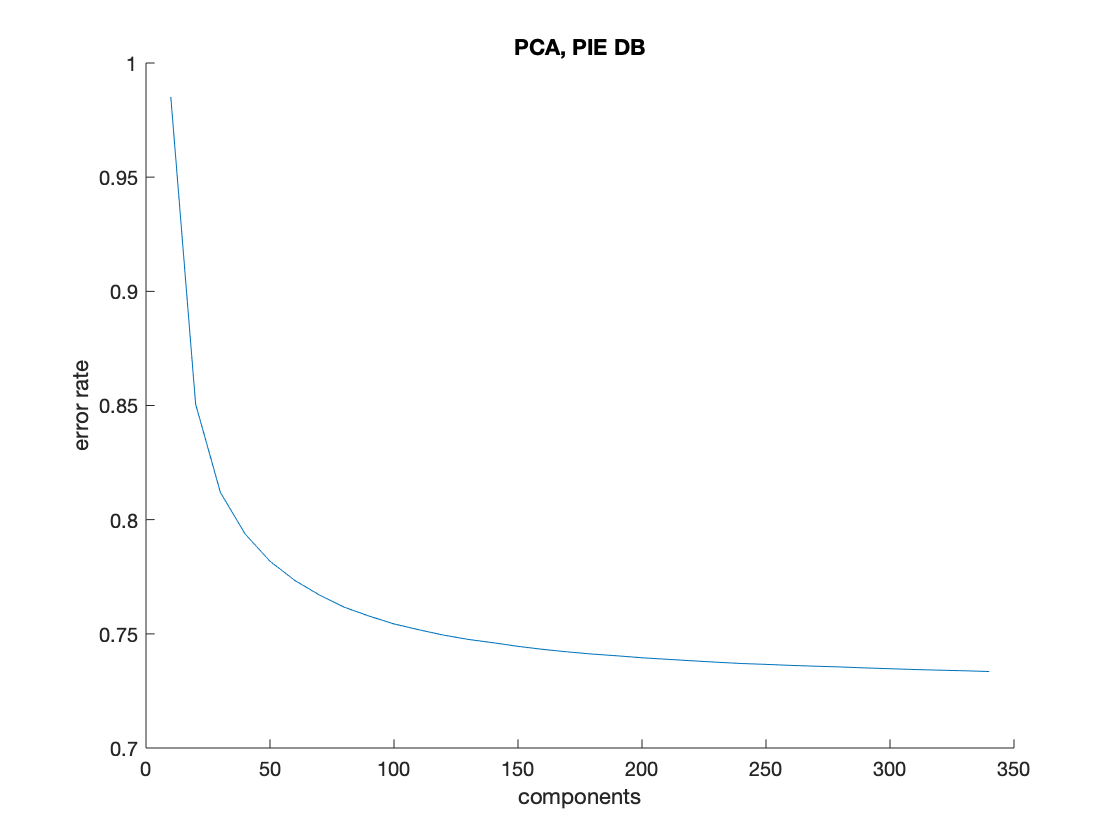
\includegraphics[width = 0.8\hsize]{./figures/pca.png}
    \caption[...]{Error rate vs number of components used in model, after extracting features using PCA. Error rate is classification error rate for facial recognition protocol using KNN with features as the components extracted after preforming PCA.}
    \label{fig:pca}
\end{figure}

\begin{figure}[H]
    % \ContinuedFloat*
    \centering
    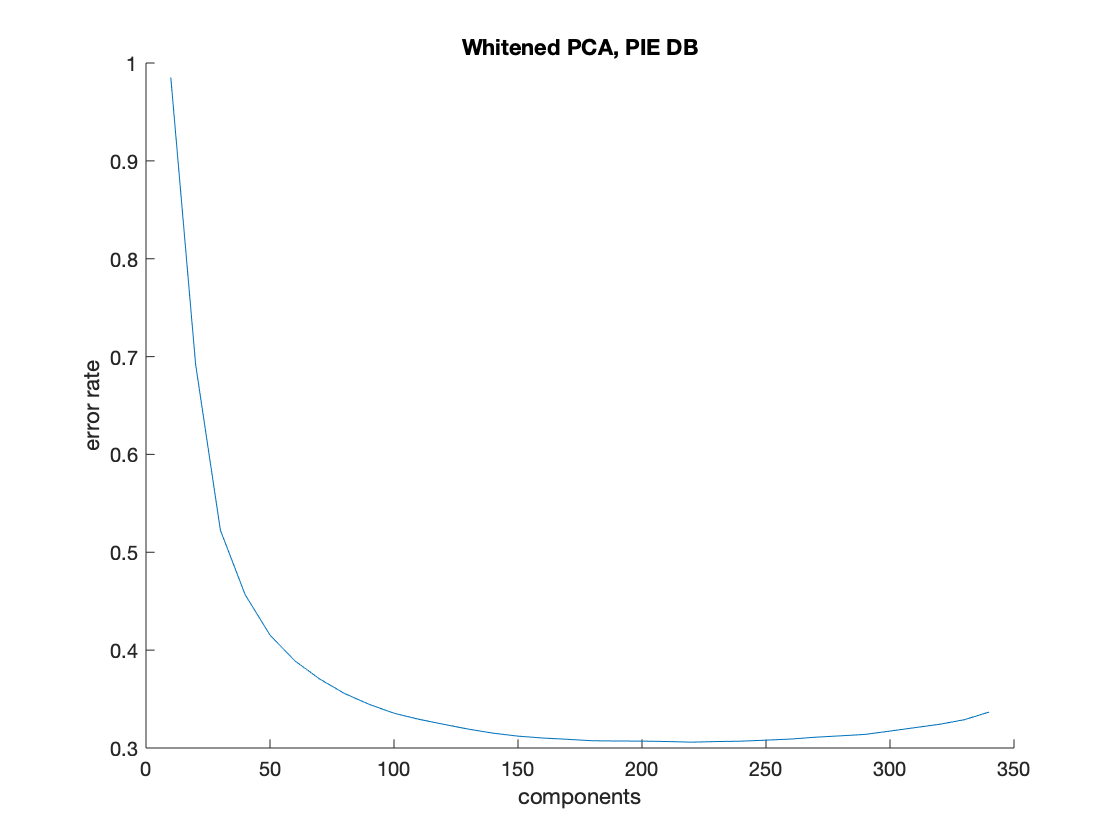
\includegraphics[width = 0.8\hsize]{./figures/wpca.png}
    \caption[...]{Equivalent to \autoref{fig:pca} but using whitened PCA to extract features.}
    \label{fig:wpca}
\end{figure}

\begin{figure}[H]
    % \ContinuedFloat*
    \centering
    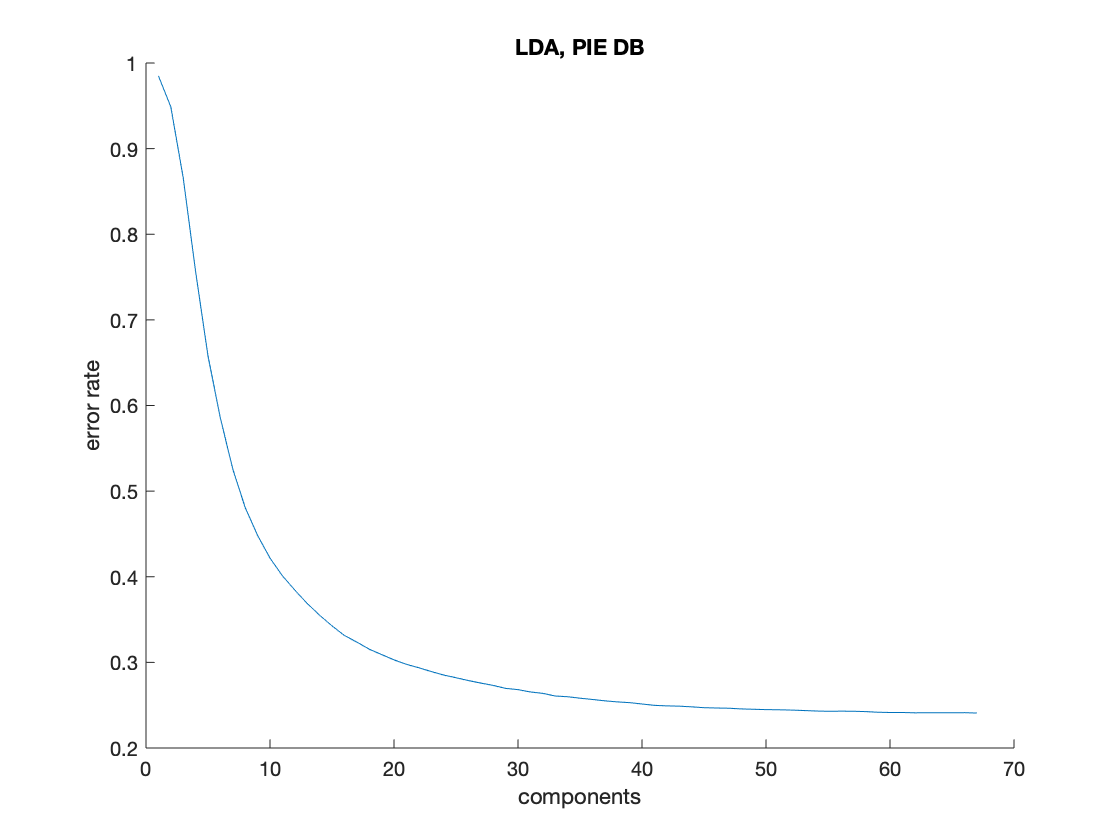
\includegraphics[width = 0.8\hsize]{./figures/lda.png}
    \caption[...]{Equivalent to \autoref{fig:pca} but using LDA to extract features.}
    \label{fig:lda}
\end{figure}

\newpage
\section{}

\subsection{}

The Lagrangian can be formulated as:
\begin{align}
    \mathcal{L}(\mathbf{w}, b, \xi, a_i, r_i) = \frac{1}{2} \mathbf{w^{\top} S_t w} + C \sum_{i=1}^{n} \xi_i - \sum^n_{i=1}a_i (y_i(\mathbf{w^{\top} x_i} + b) - 1 + \xi) -\sum_{i=1}^n r_i\xi_i
\end{align}

Taking derivatives and setting equal to zero:
\begin{align}
     & \frac{\partial \mathcal{L}}{\partial \mathbf{w}} = \mathbf{w S_t} -  \sum^n_{i=1} a_i y_i \mathbf{x_i} = 0 \iff \mathbf{w_0} = \mathbf{S_t}^{-1}  \sum^n_{i=1} a_i y_i \mathbf{x}_i
     \\
     & \frac{\partial \mathcal{L}}{\partial b} = \sum^n_{i=1} a_i y_i = 0
     \\
     & \frac{\partial \mathcal{L}}{\partial \xi_i} = C - a_i - r_i = 0
\end{align}

Substituting these back in we get the dual problem:
\begin{align}
    & \max_\mathbf{a} \mathcal{L} (\mathbf{a}) = \mathbf{a^\top 1} - \frac{1}{2} \mathbf{a^\top K}_y \mathbf{a}
    \\
    & \text{subject to } \mathbf{a} ^\top \mathbf{y} = 0, 0 \leq a_i \leq C
\end{align}

Where $\mathbf{K}_y = [y_i y_j \mathbf{x}_i^\top \mathbf{S_t}^{-1} \mathbf{x}_j]$. \\

Optimal $b$ can be found by first considering the complementary slackness condition:
\begin{align}
    a_i > 0 \implies y_i(\mathbf{w_0^\top x_i} + b) = 1
\end{align}
This means we can find optimal $b, b_0$ from any support vector. A more stable solution can be found by taking the average over all support vectors:
\begin{align}
    b_0 = \frac{1}{N_\mathcal{S}} \sum_{x_i \in \mathcal{S}} (y_i - \mathbf{w^\top x_i})
\end{align}
Where $\mathcal{S}$ is the set of support vectors.
\\

We compute $\xi_i$ as follows:
\begin{align}
    \xi_i = \operatorname{max} (0, 1-y_i(\mathbf{w^\top x_i} + b) ), \quad i = 1 ,..., n
\end{align}
Optimal $\xi$ can be computed by plugging $w_0, b_0$ into this equation.


\newpage 

\subsection{}
The previous method relies upon $S_t$ being invertible. This may not be the case in small sample size problems, for example, where the number of features exceeds the number of samples. In this case, given we have 2000 samples, if each $\mathbf{x_i}$ had more than $2000$ features, we would be faced with this issue. In this case, $S_t = \mathbf{X X^\top, X} \in \mathcal{R} ^{F x F}$ would be rank deficient as its rank would be at most $n$ and its dimensions would be $F$, with $F > n$. Here $S_t$ would be singluar so the above method would fail. \\

A workaround would be to reduce the dimensions of $S_t$ first, it becomes full rank and therefore invertible. One such way would be to perform LDA first. This involves finding a transformation so to maximise the separability of different classes in a low-dimensional latent space while also minimizing the variance of samples from the same class. This reduces the dimensions of $\mathbf{S_t}$ to at most $C-1$ with C being the number of classes (2 in this case). We could then solve the SVM problem as detailed above to obtain an SVM classifier because the new scatter matrix is invertible. \\

This approach of first running LDA could be conducted as follows:

\begin{enumerate}
    \item Perform whitening on $\mathbf{S_t}$ (i.e. compute $\mathbf{U = X(I-M)V_w \Lambda_w^{-1}}$)
    \item Compute projected data $\mathbf{\Tilde{X_b} = U^\top XM}$
    \item Perform eigenanalysis on $\mathbf{\Tilde{X_b}^\top \Tilde{X_b} = Q\Lambda_bQ^\top}$
    \item Compute the final transformation $\mathbf{W_0 = UQ_0}$
\end{enumerate}

Now we could use our SVM classifier using our transformed dataset comprising of $\mathbf{\Tilde{X}} \in \mathcal{R}^{n x (C-1)}$ knowing that $\mathbf{\Tilde{X} \Tilde{X}^\top}$ is full rank. In this case $C = 2$ so $\mathbf{\Tilde{X} \Tilde{X}^\top} \in \mathcal{R}$, hence the new scatter matrix would be a scalar, therefore it is invertible. \\


\end{document}
%%% Local Variables: 
%%% mode: latex
%%% TeX-master: t
%%% End: 
